\documentclass[aspectratio=169]{beamer}

\usepackage{amsmath}
\usepackage{amssymb}
\usepackage[T1]{fontenc}
\usepackage{graphicx}
\usepackage{natbib}

\definecolor{purpledark}{RGB}{72, 12, 120}
\definecolor{purplemid}{RGB}{120, 40, 180}
\definecolor{purplelight}{RGB}{180, 130, 220}

\usetheme{Madrid}
\usecolortheme[named=purpledark]{structure}

\setbeamercolor{palette primary}{bg=purpledark, fg=white}
\setbeamercolor{palette secondary}{bg=purplemid, fg=white}
\setbeamercolor{palette tertiary}{bg=purplelight, fg=white}
\setbeamercolor{palette quaternary}{bg=purpledark, fg=white}
\setbeamercolor{title}{fg=purpledark}
\setbeamercolor{frametitle}{fg=purpledark, bg=white}
\setbeamercolor{normal text}{fg=black}
\setbeamercolor{block title}{bg=purplemid, fg=white}
\setbeamercolor{block body}{bg=purplelight!15!white, fg=black}

\setbeamertemplate{navigation symbols}{}

\title{Machine Learning Stellar Classification}
\subtitle{Rediscovering the HR Diagram}
\author{Krupa Pothiwala}
\institute{Florida Institute of Technology}
\date{May 2026}
\setbeamertemplate{title page}{
  \begin{beamercolorbox}[wd=\paperwidth, ht=2.5em, dp=0.8em, center]{frametitle}
    \usebeamerfont{title}\inserttitle
  \end{beamercolorbox}
  \begin{center}
    \usebeamerfont{subtitle}\textit{\insertsubtitle}\\[0.5em]
    \vfill
    \usebeamerfont{author}\insertauthor\\[0.5em]
    \usebeamerfont{institute}\insertinstitute\\[0.5em]
    \usebeamerfont{date}\insertdate
  \end{center}
  \vfill
}
\begin{document}

% Title
\begin{frame}
  \titlepage
\end{frame}

% Outline
\begin{frame}{Outline}
  \tableofcontents
\end{frame}

\section{Introduction}

\begin{frame}{The Hertzsprung-Russell Diagram}
  \begin{columns}[T]
    \begin{column}{0.48\textwidth}
      The HR diagram maps where stars are in their \textbf{life cycle}:
      \vspace{0.5em}
      \begin{itemize}
        \item \textbf{Main Sequence} - where most stars (including our Sun) spend their lives
        \item \textbf{Giants \& Supergiants} - post-main-sequence phase
        \item \textbf{Turn-off point} - stars diverge as core hydrogen runs out
        \item \textbf{White Dwarfs} - stellar remnants in the lower-left
      \end{itemize}
    \end{column}
    \begin{column}{0.48\textwidth}
      \centering
      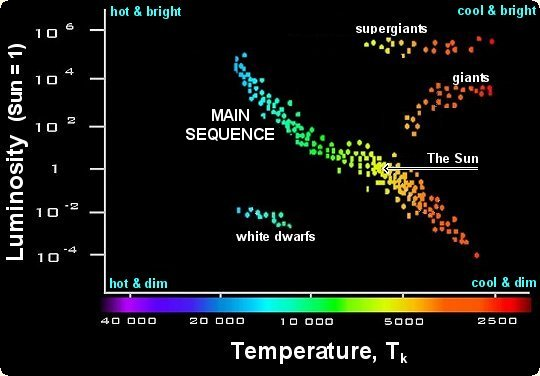
\includegraphics[width=\linewidth]{hrdiagram_01.jpg}
      \vspace{1em}
    \end{column}
  \end{columns}
\end{frame}

\begin{frame}{Conventional Definition}
    There are certain terms that would be useful to know going forward \\[0.5em]
    \begin{itemize}
        \item mas - milli arcsecond (angular measurement). Take a full circle of 360 degrees and one degree is 60 arcminutes so one arcsecond is 1/3600th of degree.
        \item G band - G filter on the telescope, measures white light ($330-1050 nm$)
        \item parsec ($\varpi$) - unit of length used in astronomy. 3.26 light years $\approx$ 1 parsec
        \item parallax - distance measurements (mas). Formula used for it is parsecs $=1000/\varpi$.
        \item apparent magnitude ($m$) - brightness as it appears to us. Depends on the band.
        \item Absolute magnitude ($M$) - brightness of the object if it was 10 parsecs away from Earth. Normalized magnitude. Depends on the band
        \item Extinction ($A$) - how much light gets absorbed between us and the object. Depends on the band.
    \end{itemize}
\end{frame}

\begin{frame}{Research Question}
  \begin{center}
    \Large
    Can unsupervised machine learning \textbf{rediscover} the structure of the HR diagram from raw, unlabelled stellar data \textit{with no prior knowledge of stellar physics?}
  \end{center}
\end{frame}

\section{Data}

\begin{frame}{Data: Gaia DR3, NGC 2516}
  \begin{columns}[T]
    \begin{column}{0.48\textwidth}
      \textbf{Source:} ESA Gaia Data Release 3 \cite{gaia_dr3} and \cite{gaia_archive} \\[0.5em]
      Retrieved via \texttt{astroquery.gaia} (Python) \cite{astroquery_gaia} \\[1em]
      \textbf{Cone Search Parameters:}
      \begin{itemize}
        \item RA $= 119.517^{\circ}$, Dec $= -60.752^{\circ}$
        \item Radius: $1.0^{\circ}$
        \item Parallax: $1.5$--$3.5$ mas
        \item $\mu_\alpha = -4.7 \pm 3.0$ mas/yr
        \item $\mu_\delta = 11.2 \pm 3.0$ mas/yr
        \item Parallax error $< 0.5$ mas
      \end{itemize}
    \end{column}
    \begin{column}{0.48\textwidth}
      \textbf{Columns Retrieved:}
      \begin{itemize}
        \item Apparent magnitudes ($G$, BP, RP)
        \item Color indices
        \item Proper motions
        \item Parallax
        \item Extinction estimates
      \end{itemize}
      \vspace{1em}
      \begin{block}{Final Sample}
        \centering \large \textbf{2,670 member stars}
      \end{block}
    \end{column}
  \end{columns}
\end{frame}

\section{Data Cleaning}

\begin{frame}{Data Cleaning \& Feature Engineering}
  \begin{columns}[T]
    \begin{column}{0.48\textwidth}
      \textbf{Cleaning Steps:}
      \begin{enumerate}
        \item Drop rows missing $m_G$, $\varpi$, BP$-$RP, $\mu$
        \item RUWE quality cut: remove RUWE $\geq 1.4$ \cite{pearce2022ruwe}
        \item Drop columns with $>60\%$ missing values
        \item Remove GSP-Phot (General Stellar Parametrizer from Photometry) columns (too incomplete). 
      \end{enumerate}
    \end{column}
    \begin{column}{0.48\textwidth}
      \textbf{Derived Features:}\\[0.8em]
      \textit{Absolute Magnitude:}
      \[
        M_G = m_G - 5\log_{10}(d) + 5 - A_G
      \]
      where $d\,[\text{pc}] = 1000/\varpi$\\[1em]
      \textit{Corrected Color Index:}
      \[
        (BP-RP)_0 = (BP-RP) - E(BP-RP)
      \]
      Removes interstellar reddening.
    \end{column}
  \end{columns}
\end{frame}

\section{Machine Learning}

\begin{frame}{Machine Learning Pipeline}
  \begin{block}{Features (4 inputs)}
    Apparent magnitudes: $m_G$,\; $m_{BP}$,\; $m_{RP}$ \quad + \quad Parallax: $\varpi$
  \end{block}
  \vspace{0.5em}
  \begin{enumerate}
    \item \textbf{Z-score Normalisation}: rescale each feature to mean $0$, std $1$
    \item \textbf{PCA}: compress 4 features into 2 principal components
    \item \textbf{UMAP + HDBSCAN}: explored, but discarded
  \end{enumerate}
  \vspace{0.5em}
  \begin{alertblock}{Why not UMAP + HDBSCAN?}
    HDBSCAN traced UMAP's layout, not real data structure; \textbf{pipeline bias}. PCA alone was sufficient.
  \end{alertblock}
\end{frame}

\section{Results}

\begin{frame}{Results: PCA Output}
  \textbf{99.7\% of total variance} captured in 2 components\\[1em]
  \begin{columns}[T]
    \begin{column}{0.48\textwidth}
      \textbf{PC1 - Brightness Gradient}
      \begin{itemize}
        \item Traces the full main sequence
        \item Hot blue stars at one end, faint red stars at the other
        \item Giants separate naturally at negative PC1
      \end{itemize}
    \end{column}
    \begin{column}{0.48\textwidth}
      \textbf{PC2 - Residual Scatter}
      \begin{itemize}
        \item Near-constant along the main sequence
        \item Picks up parallax depth / cluster spread
        \item No new astrophysical information
      \end{itemize}
    \end{column}
  \end{columns}
  \vspace{0.8em}
  \begin{block}{}
    \centering The model recovered HR diagram structure \textbf{entirely without supervision}.
  \end{block}
\end{frame}

\begin{frame}{Result Visualization}
    \begin{figure}
        \centering
        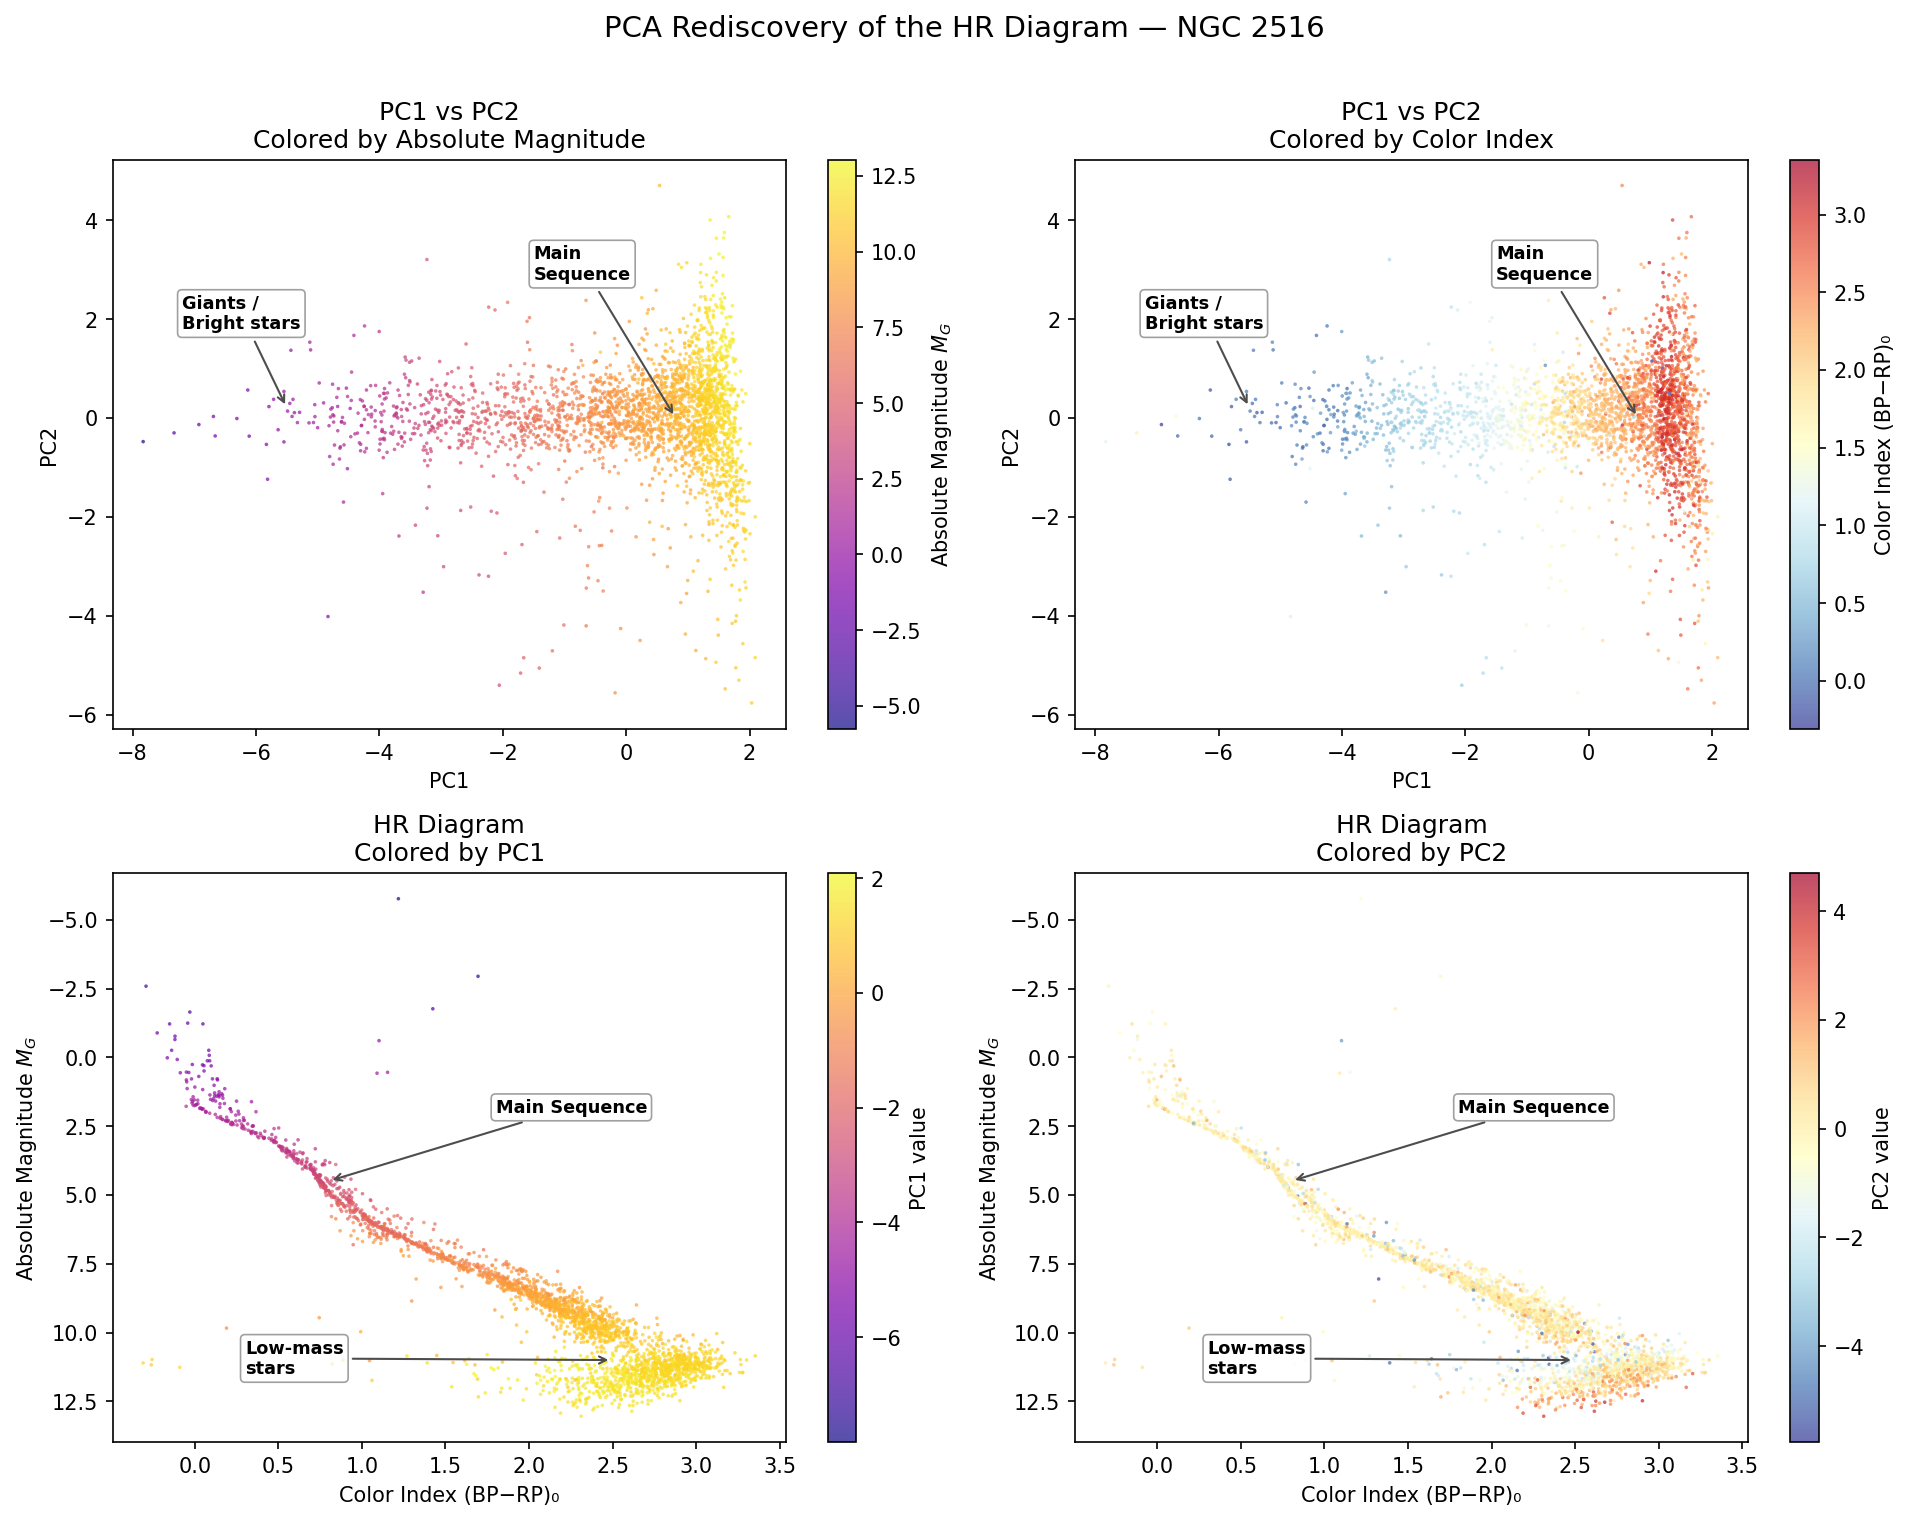
\includegraphics[width=9.0cm]{hr_diagram_pca.png}
        \caption{PCA HR Diagram}
        \label{fig:placeholder}
    \end{figure}
\end{frame}
\section{Conclusion}

\begin{frame}{Conclusion}
  \begin{itemize}
    \item PCA recovered the HR diagram from raw photometric data with \textbf{no prior physics knowledge}
    \item 2 components captured \textbf{99.7\%} of variance; almost no information lost
    \item PC1 $\equiv$ brightness / main sequence axis; PC2 $\equiv$ residual scatter
    \item UMAP + HDBSCAN introduced pipeline bias - complexity is not always better
  \end{itemize}
  \vspace{1em}
  \begin{block}{Broader Insight}
    Stellar physics is structured enough that a simple linear model can rediscover fundamental
    astronomical relationships from scratch, given the right raw data.
  \end{block}
\end{frame}

\begin{frame}{References}
    \scriptsize
    \setlength{\bibsep}{16pt}
    \bibliographystyle{apalike}
    \bibliography{references}
\end{frame}


\end{document}
